\documentclass[multi,preview,varwidth=false,border=5,12pt]{standalone}
%\documentclass[12pt]{article}

\newcounter{Qnum}
\usepackage{assignments}
\standaloneenv{question}


\excludecomment{solution}\let\endsolution\relax


\begin{document}

\begin{center}
\section*{Flow of fluids}
\end{center}

\begin{question}

A tank contains 8733 lbs of water at room temperature. How many hours would it take to empty the tank if a pump removes 2.5 gallons of water from the tank every minute.

\begin{solution}

First, let's figure out how many gallons of water we have.

\begin{align*}
    V=\frac{w}{\gamma}=\frac{8733~\lb}{62.21~\lb/\ft^3}=140.4~\ft^3\times\left(\frac{7.48~\gal}{\ft^3}\right)=1050~\gal
\end{align*}

If we remove 2.5 gallons of water every minute it would take

\begin{align*}
    \left(1050~\gal\right)/(2.5~\gal/\min) = 420 ~\min \times \left(\frac{1~\hr}{60~\min}\right)=7~\hr
\end{align*}

\end{solution}

\end{question}


\begin{question}

If 400 L/min of fluid flows through a DN 50 Schedule 80 steel pipe what is the resulting average velocity (in m/s) of flow?

\begin{solution}
\end{solution}

\end{question}


\begin{question}

What is the smallest size standard Schedule 40 steel pipe that would carry 2.80 L/min of oil with a an average flow velocity below 0.3 m/s?  Report your answer as a metric Nominal Pipe Size (DN).

\begin{solution}
\end{solution}

\end{question}



\begin{question}

An aneurysm is an abnormal enlargement of a blood vessel such as the aorta.  A  patient's abdominal CT scan reveals an abnormal abdominal aortic diameter of $5.0~\cm$ compared to their normal aortic diameter of $2.5~\cm$.  If blood of density $1060~\kg/\m^3$ travels through the normal portion of the aorta at a speed of $40~\cm/s$ by how much does the pressure in the abnormal region exceed that of the normal region?  Report your answer in kPa.

\begin{solution}
\end{solution}

\end{question}



\begin{question}

Turpentine is flowing at $0.45~\m^3/s$ in the fabricated tube shown below.  If the pressure before the enlargement at A is 500 kPa what is the pressure at point B?

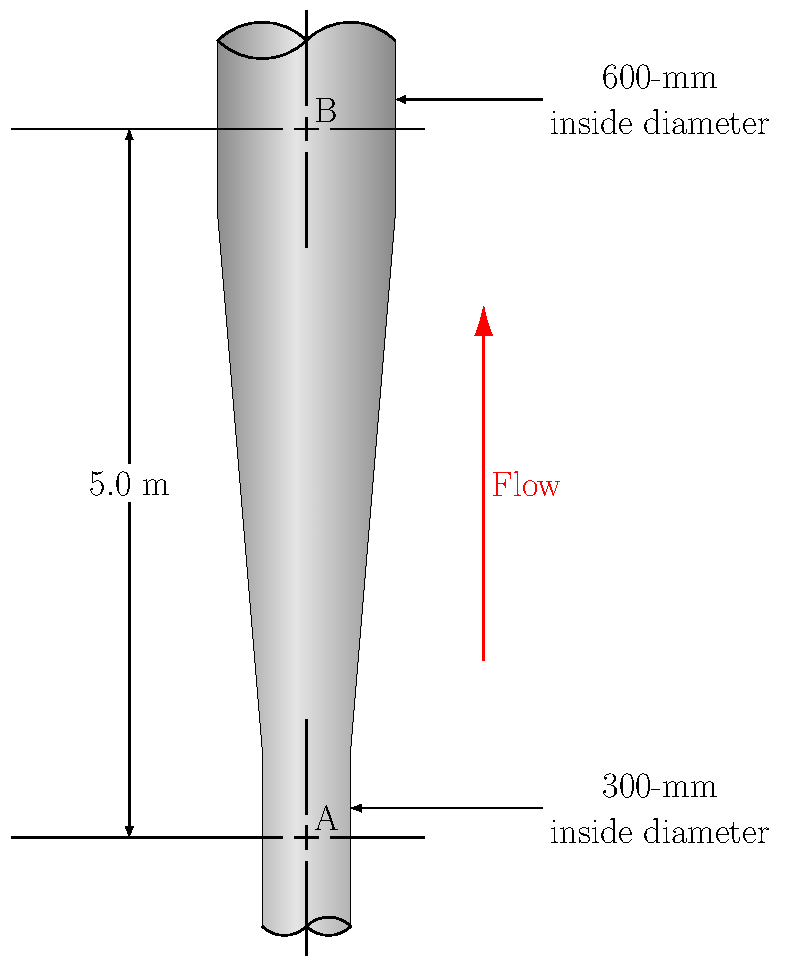
\includegraphics[width=3in]{imgs/PipeExp1.pdf}


\begin{solution}
\end{solution}

\end{question}


\begin{question}

Octane is flowing at 10 gpm from a standard 1-in Schedule 40 steel pipe to a standard 2-in Schedule 40 steel pipe.  The pipes are horizontal.  What is the difference in pressure (in psi) between the two pipes?

\begin{solution}
\end{solution}

\end{question}



\end{document}
